\documentclass[border=1pt]{standalone}

\usepackage[T1]{fontenc}
\usepackage{newtxtext}
\usepackage{graphicx}
\usepackage{tikz}
\usetikzlibrary{arrows.meta,calc,fit,positioning}

\begin{document}

\resizebox{7.16in}{!}{%
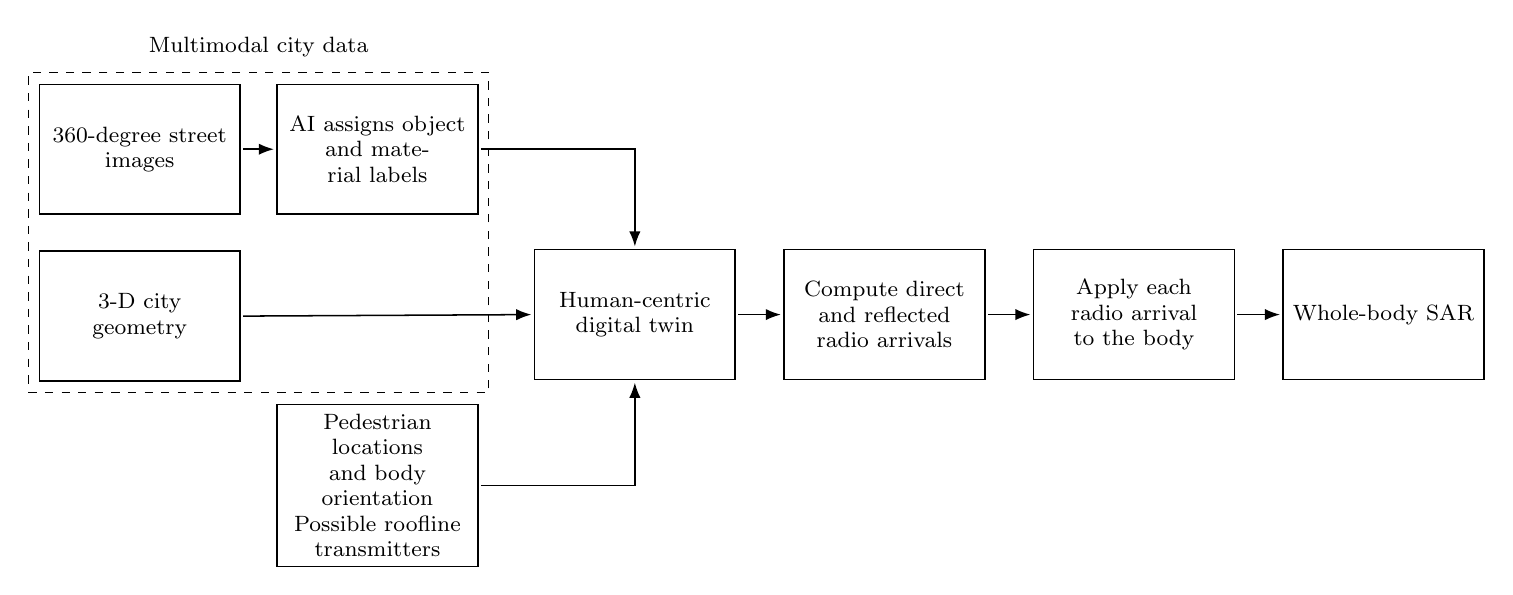
\begin{tikzpicture}[
  every node/.style={
    font=\fontsize{8.1}{9.2}\selectfont,
    text=black
  },
  block/.style={
    draw=black,
    line width=0.55pt,
    rectangle,
    fill=white,
    align=center,
    inner xsep=1.1mm,
    inner ysep=1.2mm,
    minimum width=25.5mm,
    minimum height=16.5mm,
    text width=23.3mm
  },
  arrow/.style={
    ->,
    draw=black,
    line width=0.55pt,
    >=Latex,
    shorten <=0.3mm,
    shorten >=0.3mm
  }
]
  \node[block] (images) {360-degree street\\images};
  \node[block, below=4.5mm of images] (geometry) {3-D city\\geometry};
  \node[block, right=4.5mm of images] (labels)
    {AI assigns object\\and material labels};
  \node[block, below=24mm of labels] (setup)
    {Pedestrian locations\\and body orientation\\Possible roofline\\transmitters};

  \node[block, right=7.0mm of labels, yshift=-21mm] (twin)
    {Human-centric\\digital twin};
  \node[block, right=6.0mm of twin] (arrivals)
    {Compute direct\\and reflected\\radio arrivals};
  \node[block, right=6.0mm of arrivals] (body)
    {Apply each radio arrival\\to the body};
  \node[block, right=6.0mm of body] (sar)
    {Whole-body SAR};

  \draw[arrow] (images) -- (labels);
  \draw[arrow] (labels.east) -| (twin.north);
  \draw[arrow] (geometry.east) -- (twin.west);
  \draw[arrow] (setup.east) -| (twin.south);
  \draw[arrow] (twin) -- (arrivals);
  \draw[arrow] (arrivals) -- (body);
  \draw[arrow] (body) -- (sar);

  \node[
    draw=black,
    dashed,
    line width=0.45pt,
    inner xsep=1.3mm,
    inner ysep=1.4mm,
    fit=(images)(geometry)(labels)
  ] (multimodal) {};
  \node[
    anchor=south,
    yshift=0.7mm,
    font=\fontsize{7.7}{8.7}\selectfont
  ] at (multimodal.north) {Multimodal city data};
\end{tikzpicture}%
}

\end{document}
